%!TEX root = thesis.tex

\chapter{Gesture Recognition}
\label{ch:gestures}

Knowing the location of the hands in a image doesn't tell much about the hand poses. A method needs to be constructed to discriminate the different hand poses.

This chapter describes how the hand poses are detected in the hand windows. Features are extracted from the hand window and represent the hand pose in a more compact way. These features are compared by a classifier with previously extracted features of hand poses for which the labels are known. The classifier will determine which known hand pose(s) resembles the at that moment examined hand.


\section{Feature extraction}
The hand window contains some background pixels, because a hand will never fill a perfect square (Figure \autoref{fig:lefthandwindow}). These pixels are unwanted since they contain arbitrary values that introduce noise into our process. In \autoref{sec:skinmodel} a binary mask for skin pixels is constructed. The inverse skin mask can be used  to remove the background (Figure \autoref{fig:lefthandcutout}). Sometimes the blob is too small to say something useful about the hand pose. One way to artificially increase the blob size is to do a morphological dilate operation on the blob. This will increase the size of the hand cutout and probably add skin pixels, but this will also introduce more noisy (non-skin) pixels.

To compare two or more hands with each other a method is required to calculate the similarity. A very simple method is to compare each pixel location with each other and sum all the differences. But this method isn't feasible. It is not going to work on images that are not the same size or orientation. Also it is computationally expensive for larger images - for an image of 100 by 100 pixels there are already 10.000 dimensions. Also important is that this method is not very forgiving for small variations like scaling and rotation.


\begin{figure}[htbp]
\begin{center}
\subfloat[Hand window]{
        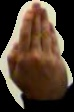
\includegraphics[width=0.2\linewidth]{figures/pipeline/lefthand.jpg}
        \label{fig:lefthandwindow}
}
\hspace{0.03\linewidth}
\subfloat[Hand cutout]{
        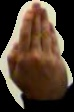
\includegraphics[width=0.2\linewidth]{figures/pipeline/lefthandcutout.jpg}
        \label{fig:lefthandcutout}
}
\hspace{0.03\linewidth}
\subfloat[Resized hand, used for feature extraction]{
        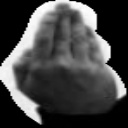
\includegraphics[width=0.2\linewidth]{figures/pipeline/lefthandhog.jpg}
        \label{fig:lefthandfeatures}
}
\caption{Preparing the hand window for feature extraction}
\label{fig:featureprep}
\end{center}
\end{figure}

\subsection*{Descriptors}
To reduce the number of dimensions of an image a descriptor can be used. A descriptor describes an image in, if properly used, less dimensions than the image itself. Also it can introduce some useful properties like scale and rotation invariance. In this paper 2 descriptors are discussed and compared, Histogram of oriented gradient\cite{NavneetDalal2006} (HOG) and Speeded Up Robust Features\cite{Bay2006} (SURF).

The HOG descriptor has been successfully applied and studied in human detection \cite{NavneetDalal2006, watanabe2009}. The HOG descriptors method uses a dense grid of uniformly spaced cells, where for each cell the gradients are calculated in 9 orientations. The values for each orientation for each cell are stored in a histogram that represent the image. \autoref{fig:hog} visualizes a simplification of the HOG calculation. 

\begin{figure}[htbp]
\center{}
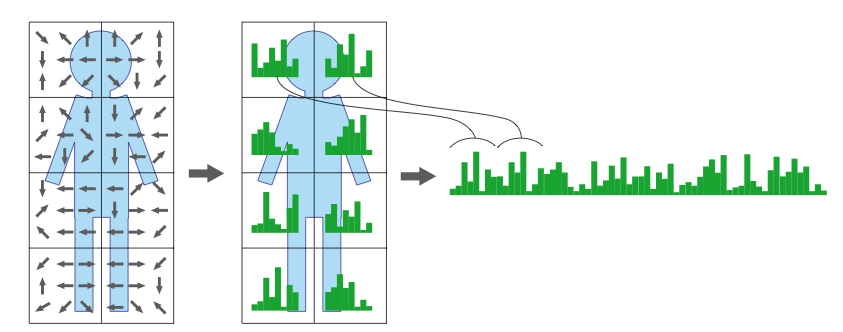
\includegraphics[width=0.8\linewidth]{figures/hog.png}
\caption{Visual representation of HOG calculation}
\label{fig:hog}
\end{figure}


The SURF descriptor is based on sums of approximated 2D Haar wavelet responses and makes use of integral images. SURF approximates the speed of Scale-invariant feature transform (SIFT) and is claimed to more robust against several image transformations\cite{Murillo2007, Valgren2010}. SIFT is an other descriptor that is often used. SIFT is similar to HOG as in they both build a histogram of gradients of the keypoints. SIFT and SURF differ from HOG in that they incorporate a method for calculating usable key points, HOG uses a dense grid of key points.



\subsection{Principal Component Analysis}
Principal Component Analysis (PCA) is a method that reduces data dimensionality by performing a covariance analysis between vectors. The original space will be mapped into a new space based on the variance in the original data. PCA transforms a number of correlated variables into a (possibly smaller) number of uncorrelated variables called principal components. The first principal component vector accounts for as much of the variability in the data as possible, and each consecutive component vector accounts for as much of the remaining variability as possible. 

PCA may improve the performance of a classifier both in classification and time performance.

\section{Classification}
Using a set of training examples each marked as belonging to a category, a classifier builds a model that predicts whether a new example falls into one category or the other. There are many classifiers which can be used in different ways. For computer vision two of these are interesting because of simplicity, or superiority; k Nearest Neighbors and Support Vector Machines.

\subsection*{k Nearest Neighbors}
The k-nearest neighbors algorithm (k-NN) is a method for classifying objects based on euclidean distance between training examples in the feature space. The k-nearest neighbor algorithm is one of the the simplest of all machine learning  algorithms. K-NN is a type of 'lazy learning' where all computation is deferred until classification. This results in a fast training phase, but a computationally expensive classification. Also the memory footprint is large since all data points are stored. 

The training samples are labeled multidimensional vectors. The training phase of the algorithm consists only of storing the vectors and class labels of the training samples.In the classification phase, $k$ is a user-defined constant, and an unlabeled vector is classified by assigning the label which is most frequent among the k training samples nearest to that query point.

\autoref{fig:knn} is an example of k-NN classification. The test sample (the circle) should be classified either to the squares class or to the triangles class. If $k = 3$ the circle is classified to the triangles class because there are 2 triangles and 1 square inside the inner circle. If $k = 5$ it is classified as 'square'.

\begin{figure}[htbp]
\center{}
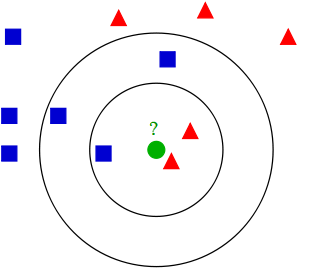
\includegraphics[width=0.5\linewidth]{figures/knn.png}
\caption{Classification using K Nearest Neighbors}
\label{fig:knn}
\end{figure}




\subsection*{Support Vector Machines}

Support vector machines (SVMs) are a set of related supervised learning methods used for classification. It is a binary classifier, but can be extended to be a multi class classifier by combining multiple binary classifiers. 

SVM uses a subset of the train data (the support vectors) that lay on the borders of a category cluster to calculate a decision boundary (DB). This DB is constructed by maximizing the distance between the support vector of two classes. The decision boundary, a linear function, is later used to classify new data points.

Often, a set of data points in a space is not linearly separable. For this reason the original space is mapped to a higher dimensional space making the separation easier. This is done by a kernel function.

The training phase consists of computing a kernel to make the space linearly separable. Then a decision boundary is calculated. Training a SVM classifier can be computationally expensive, but classification is very fast and memory efficient. The training phase has one parameter, which is the error cost $c$. $c$ controls the trade off between allowing training errors and forcing rigid margins. It is a multiplication of the error - the difference between a predicted value and true value. This allows some flexibility in separating the categories and, if properly set, prevents over and under fitting.

The function for the DB for a test sample $x$ has the following form:

\begin{equation}
	g(\mathbf{x}) = \sum_i{\alpha_i y_i K(\mathbf{x}_i,\mathbf{x}) -b},
\end{equation}

where $K(x_i,x)$ is a kernel function for the training sample $x_i$ and the test sample $x$ and $y_i$ the class label of $x_i$ with value $+1$ or $-1$. $\alpha_i$ is the weight of the training sample $x_i$ and $b$ is a threshold parameter which both are learned in the training phase.  

There are various kernels, but \cite{Hsu2003} states the Radial Basis Function is a good kernel to start with because it generally gives good results. This kernel is defined by:

\begin{equation}
	K(S_i,S_j) = e^{(-\gamma||S_i-S_j||^2)}, \gamma > 0,
\end{equation}

where $S_i$ and $S_j$ are two feature vectors. It has one parameter $\gamma$ which needs adjusting to fit the dataset, it controls the scale of the kernel. An other interesting kernel is based upon the $\chi^2$ distance\cite{Zhang2007}. An advantage is that it doesn't have a parameter that needs optimization. This distance is incorporated into SVM by the usage of Gaussian kernels\cite{Chapelle1999}:

\begin{equation}
	K(S_i,S_j) = exp(-\frac{1}{A}D(S_i,S_j)),
\end{equation}

where $D(S_i,S_j)$ is defined as

\begin{equation}
	D(S_1,S_2) = \frac{1}{2}\sum^{m}_{i=1}\frac{(u_i-w_i)^2}{u_i+w_i},
\end{equation}

with $S_1 = \{u_1, ... , u_m\}$ $S_2 = \{w_1, ... , w_m\}$.

\autoref{fig:svm} is an example of a SVM classification setting. The space is already linearly separable, so no space transformation is required. 

\begin{figure}[htbp]
\center{}
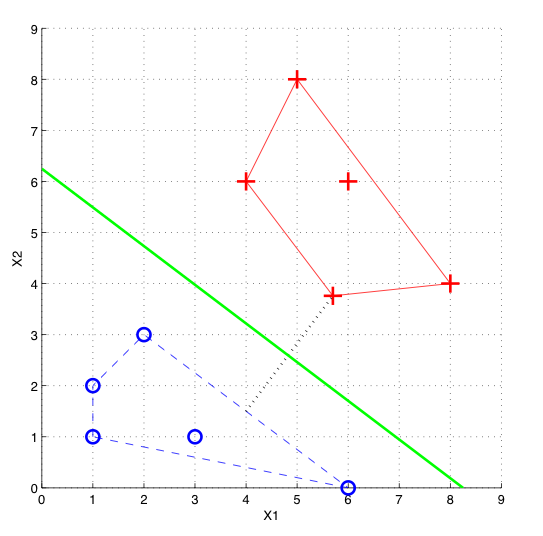
\includegraphics[width=0.5\linewidth]{figures/svm2.png}
\caption{Classification using Support Vector machines}
\label{fig:svm}
\end{figure}




\subsection*{The stabilizer}
\label{subsec:stabilizer}
Since consecutive frames in a video sequence have a spatial-temporal relationship their labels have this property also. Because of noise, misclassification can happen. These false matches can be filtered out by smoothing the labels on a time scale.

This smoothing is done with a simple self invented method called 'the stabilizer'.

A visual representation is given in \autoref{fig:stabilizer}. The stabilizer is initialized with $n$ numbers of bins which is equal to the number of labels. There are 2 parameters, $V_{max}$ which controls the maximum and $V_{th}$ which controls the threshold.

For every new label that is given by the classifier all bins are decremented with 1, except for the bin with the currently classified label which is incremented. A bin is incremented until it reaches $V_{max}$. When at any moment one of the bins value rises above $V_{th}$, the stabilizer will output the label of that bin. The result is a more stable and smoothed stream of labels, where single noisy labels are filtered out. For a sequence of frames with a correctly detected pose there is a delay between the first frame and the stabilizer will output the correct label, this delay is controlled by $V_{th}$ which is measured in frame count. A higher value will reduce more noise, but will give a bigger delay. There is also a delay after a sequence which is controlled by $n_{max}$. With a framerate between $10$ and $25$ frames a second, $V_{max} = 15$ and $V_{th} = 10$ give good results reducing noise and still being very responsive.

\begin{figure}[htbp]
  \centering
\subfloat[A]{
    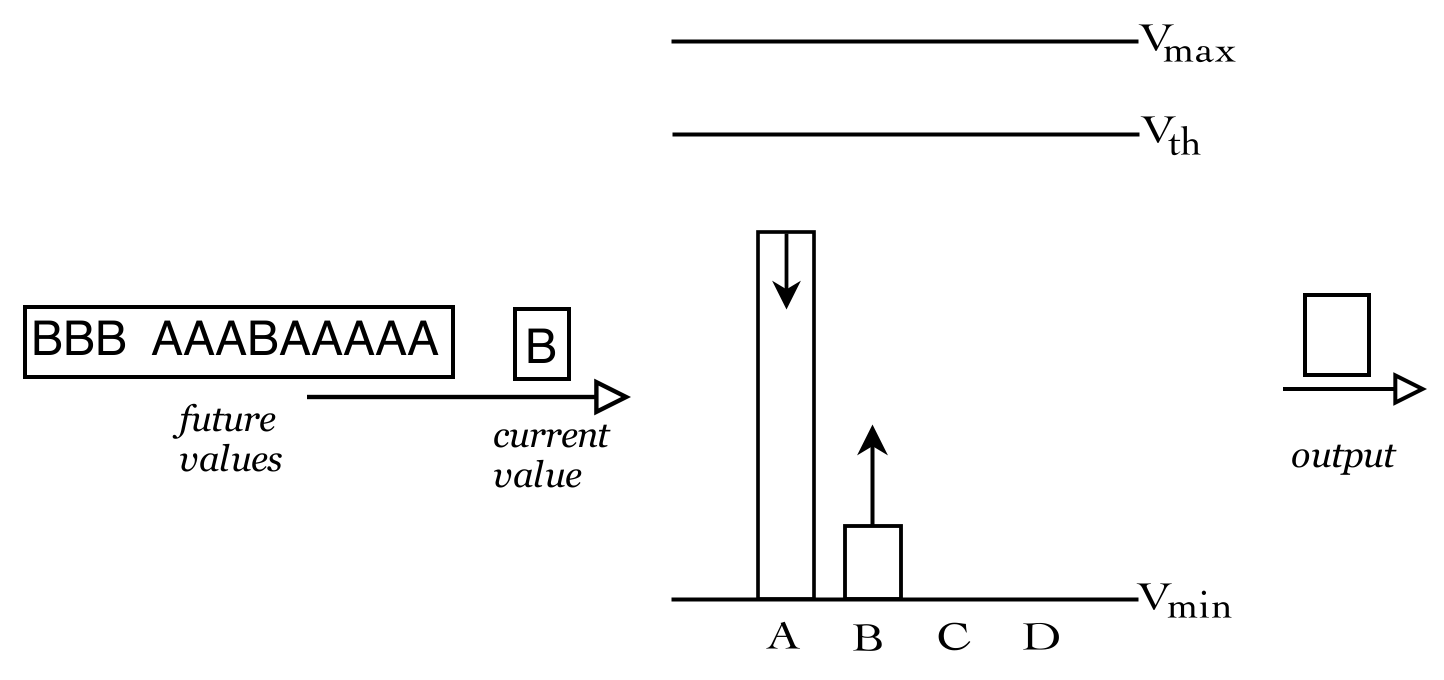
\includegraphics[width=0.7\textwidth]{figures/stabilizer/b.png}
}
\hspace{0.03\linewidth}
\subfloat[B]{
    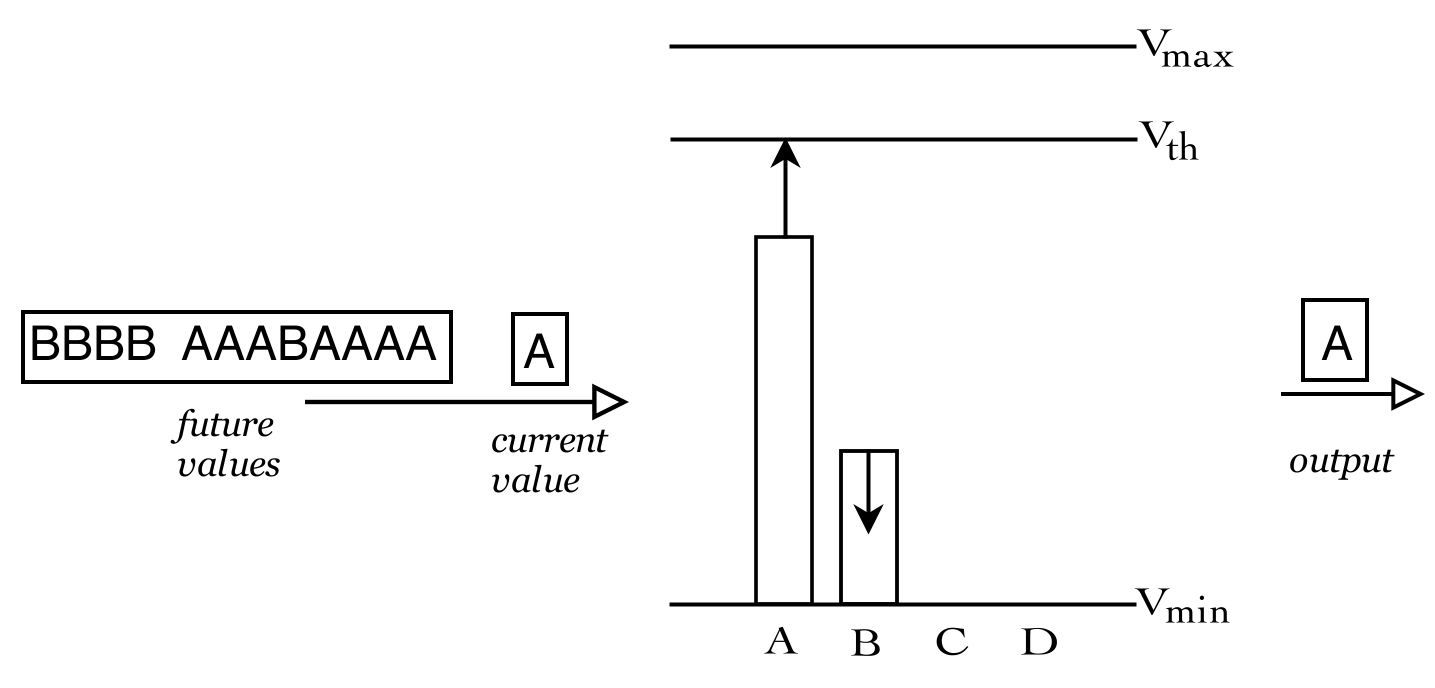
\includegraphics[width=0.7\textwidth]{figures/stabilizer/a.png}
}
  \caption{Two examples of a stabilizer in action}
  \label{fig:stabilizer}
\end{figure}

